% Compile with pdflatex (the figures are drawn with TikZ: no shell escape,
% no PSTricks, no Ghostscript post-processing).

\documentclass[aspectratio=169]{beamer}

\usepackage[utf8]{inputenc}
\usetheme{Singapore}
\usepackage{xcolor}
\setbeamertemplate{footline}[frame number]

\usepackage{algorithmicx}
\usepackage{algpseudocode}

\usepackage{amsmath,amssymb,amsthm}

\usepackage{tikz}
\usetikzlibrary{arrows.meta,positioning,calc}

\usepackage{graphicx}

\setbeamercovered{dynamic}

\def\DD{\mathcal{D}}
\def\EE{\mathbb{E}}
\def\QQ{\mathcal{Q}}

%---------------------------------------------------------------- tree styles
\tikzset{
  nd/.style      = {circle, draw, minimum size=4.5mm, inner sep=0pt,
                    line width=0.6pt, font=\scriptsize},
  ndsel/.style   = {nd, draw=red, line width=1.2pt},
  ndleaf/.style  = {circle, fill=black, minimum size=1.4mm, inner sep=0pt},
  edg/.style     = {line width=0.6pt},
  edgsel/.style  = {draw=red, line width=1.8pt},
  edgd/.style    = {line width=0.5pt, dashed},
  sib/.style     = {line width=0.6pt, dotted},
  stg/.style     = {font=\scriptsize},
}

% Three-stage scenario tree used in the nested decomposition illustrations.
% #1/#2: style and content of the stage-1 node, #3: label below that node,
% #4/#5: style and content of the stage-2 nodes,
% #6/#7: style and content of the stage-3 nodes.
\newcommand{\nlsdtree}[7]{%
\begin{tikzpicture}[scale=0.88]
  \node[#1] (r)  at (0,0)      {#2};
  \node[stg] at (0,-0.55) {#3};
  \node[#4] (a1) at (2.4,1.2)  {#5};
  \node[#4] (a2) at (2.4,-1.2) {#5};
  \node[#6] (b1) at (4.8,1.8)  {#7};
  \node[#6] (b2) at (4.8,0.6)  {#7};
  \node[#6] (b3) at (4.8,-0.6) {#7};
  \node[#6] (b4) at (4.8,-1.8) {#7};
  \draw[edg] (r) -- (a1) (r) -- (a2);
  \draw[edg] (a1) -- (b1) (a1) -- (b2) (a2) -- (b3) (a2) -- (b4);
  \foreach \n/\y in {b1/1.8, b2/0.6, b3/-0.6, b4/-1.8} {
    \draw[edgd] (\n) -- (6.3,\y+0.28) node[ndleaf] {};
    \draw[edgd] (\n) -- (6.3,\y-0.28) node[ndleaf] {};
  }
  \draw[sib] (a1) -- (a2);
  \draw[sib] (b1) -- (b2);
  \draw[sib] (b3) -- (b4);
  \node[stg] at (0,-2.6)   {First stage};
  \node[stg] at (2.4,-2.6) {Second stage};
  \node[stg] at (4.8,-2.6) {Third stage};
  \node[stg] at (6.3,-2.6) {$\ldots$};
\end{tikzpicture}}

% Recombining two-stage graph: every node of stage 2 is connected to every
% node of stage 3. #1/#2: styles of the stage-2 and stage-3 nodes.
\newcommand{\recombgraph}[2]{%
  \node[nd] (r) at (0,0) {$1$};
  \node[#1] (a1) at (2,1.1)  {$1$};
  \node[#1] (a2) at (2,-1.1) {$2$};
  \node[#2] (b1) at (4,1.65)  {$1$};
  \node[#2] (b2) at (4,0.55)  {$2$};
  \node[#2] (b3) at (4,-0.55) {$3$};
  \node[#2] (b4) at (4,-1.65) {$4$};
  \draw[edg] (r) -- (a1) (r) -- (a2);
  \foreach \a in {a1,a2} \foreach \b in {b1,b2,b3,b4} \draw[edg] (\a) -- (\b);}

\title[SDDP]{Stochastic optimization\texorpdfstring{\\}{: }Stochastic dual dynamic programming}

\author[Fabian Bastin]{Fabian Bastin \texorpdfstring{\\ \url{bastin@iro.umontreal.ca} \\}{, }
Université de Montréal -- CIRRELT -- IVADO -- Fin-ML}

\date{}

\begin{document}

\frame{\titlepage}

\begin{frame}
\frametitle{Context}

Introduced by Pereira and Pinto (1991), first designed to solve hydro-scheduling problems.

\mbox{}

\begin{itemize}
\item
Stochastic dynamic problem with finite horizon.
\item
Continuous, finite dimensional state and control.
\item
Convex cost, additive over stages -- we focus here on linear costs.
\item
Discrete, independent noises.
\end{itemize}

\mbox{}

Julia implementations: the \texttt{SDDP.jl} package, and the step-by-step
notebook \texttt{code/SDDP\_from\_scratch.ipynb} accompanying these slides.

\mbox{}

{\small These slides are based on Anthony Papavasiliou's material,
\url{https://ap-rg.eu/wp-content/uploads/2020/05/SDDP.pdf}.}

\end{frame}

\begin{frame}
\frametitle{Problem setting}

We consider the multistage stochastic linear program over the horizon $t = 1,\ldots, H$
(we write $H$, and not $T$, since $T$ denotes the technology matrix)
$$
\min_{x_1 \geq 0}\ c_1^T x_1 + \EE\left[ \min_{x_2 \geq 0} c_2^T x_2 + \EE\left[ \cdots +
\EE\left[ \min_{x_H \geq 0} c_H^T x_H \right] \right] \right]
$$
subject to $W_1 x_1 = h_1$ and, for $t = 2,\ldots,H$,
$$
W_t x_t = h_t(\xi_t) - T_{t-1}(\xi_t) x_{t-1}.
$$

Equivalently, in dynamic programming form, with $\QQ_{H+1} \equiv 0$,
\begin{align*}
V_t(x_{t-1}, \xi_{[t]}) &= \min_{x_t \geq 0} \left\{ c_t^Tx_t + \QQ_{t+1}(x_t, \xi_{[t]}) \ :\
W_t x_t = h_t(\xi_t) - T_{t-1}(\xi_t)x_{t-1} \right\}, \\
\QQ_{t+1}(x_t, \xi_{[t]}) &= \EE\left[ V_{t+1}(x_t, \xi_{[t+1]}) \mid \xi_{[t]} \right].
\end{align*}

{\small The expected cost-to-go is convex and piecewise linear in $x_t$: SDDP builds it
from below, one supporting hyperplane at a time (background notes). Under stagewise independence, the
conditioning disappears and a single $\QQ_{t+1}(x_t)$ serves the whole stage.}

\end{frame}

\begin{frame}
\frametitle{The nested L-shaped decomposition subproblem}

For each stage $t = 1,\ldots, H$ and node $k = 1,\ldots,N_t$ of the scenario tree, we
consider the problem $NLSD(t,k)$
\begin{align}
\min_{x_{t,k}, \theta_{t,k}}\ & c_{t,k}^T x_{t,k} + \theta_{t,k} \notag \\
\mbox{s.t. } &
W_t x_{t,k} = h_{t,k} - T_{t-1,k} x_{t-1,a(k)}, \quad (\pi_{t,k})  \notag \\
& D_{t,k,j}x_{t,k} \geq d_{t,k,j},\ j = 1,\ldots,r_{t,k}, \quad (\rho_{t,k,j}) \\
& E_{t,k,j}x_{t,k} + \theta_{t,k} \geq e_{t,k,j},\ j = 1,\ldots, s_{t,k}, \quad (\sigma_{t,k,j}) \\
& x_{t,k} \geq 0.  \notag
\end{align}
\begin{small}
\begin{itemize}
\item
$N_t$: number of nodes at stage $t$; $a(k)$: ancestor of node $k$ at stage $t - 1$;
$x_{t-1,a(k)}$: trial solution received from $a(k)$,
\item
$\theta_{t,k}$: epigraph variable approximating the cost-to-go at node $k$; $\theta_{H,k} \equiv 0$,
\item
Constraints (1): feasibility cuts, constraints (2): optimality cuts.
\end{itemize}
\end{small}

\end{frame}

\begin{frame}
\frametitle{Nested L-shaped method}

Building block: $NLSD(t, k)$, the problem at stage $t$, node $k$.
\begin{itemize}
	\item
Repeated application of the L-shaped method.
	\item
	Parent nodes send proposals for solutions to their children nodes.
\item
Child nodes send cuts to their parents.
\item
There are different sequencing protocols that determine in which
order the problems corresponding to different nodes in the
scenario tree are solved.
\end{itemize}

\end{frame}

\begin{frame}
\frametitle{Nested L-shaped method}

\begin{center}
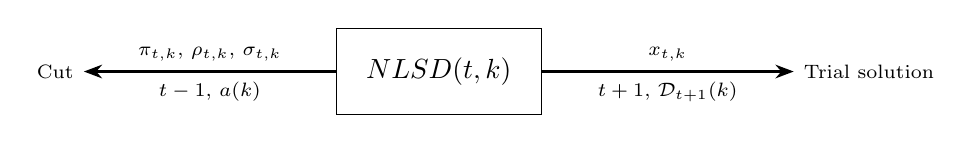
\begin{tikzpicture}[>=Stealth]
  \node[draw, minimum width=2.6cm, minimum height=1.1cm] (b) at (0,0) {$NLSD(t, k)$};
  \draw[->, line width=0.8pt] (b.west) -- node[above, font=\scriptsize] {$\pi_{t,k}$, $\rho_{t,k}$, $\sigma_{t,k}$}
                                          node[below, font=\scriptsize] {$t-1$, $a(k)$} ++(-3.2,0)
                                          node[left, font=\scriptsize] {Cut};
  \draw[->, line width=0.8pt] (b.east) -- node[above, font=\scriptsize] {$x_{t,k}$}
                                          node[below, font=\scriptsize] {$t+1$, $\DD_{t+1}(k)$} ++(3.2,0)
                                          node[right, font=\scriptsize] {Trial solution};
\end{tikzpicture}
\end{center}

\mbox{}

\begin{itemize}
	\item
$a(k)$: ancestor of node $k$.
	\item
$\DD_{t+1}(k)$: descendants of node $k$ in period $t + 1$.
\end{itemize}

\end{frame}

\begin{frame}
	\frametitle{Illustration: forward pass, stage 1}

	\begin{center}
	\nlsdtree{ndsel}{}{$x_1$}{nd}{}{nd}{}
	\end{center}

\begin{small}
\begin{itemize}
	\item
Node: $(t = 1, k = 1)$.
	\item
Direction: forward.
	\item
Output: the trial solution $x_1$, sent to every node of stage 2.
\end{itemize}
\end{small}

\end{frame}

\begin{frame}
	\frametitle{Illustration: forward pass, stage 2}

	\begin{center}
	\nlsdtree{nd}{}{$x_1$}{ndsel}{}{nd}{}
	\end{center}

	\begin{small}
	\begin{itemize}
		\item
		Node: $(t = 2, k)$, $k \in \{ 1,\ldots,N_2 \}$.
		\item
		Direction: forward.
		\item
		Output: $x_{2,k}$, $k \in \{ 1,\ldots,N_2 \}$.
	\end{itemize}
	\end{small}

\end{frame}

\begin{frame}
	\frametitle{Illustration: forward pass, stage 3}

	\begin{center}
	\nlsdtree{nd}{}{$x_1$}{nd}{}{ndsel}{}
	\end{center}

	\begin{small}
	\begin{itemize}
		\item
		Node: $(t = 3, k)$, $k \in \{ 1,\ldots,N_3 \}$.
		\item
		Direction: forward.
		\item
		Output: $x_{3,k}$, $k \in \{ 1,\ldots,N_3 \}$.
	\end{itemize}
	\end{small}

\end{frame}

\begin{frame}
	\frametitle{Illustration: backward pass, stage 3}

	\begin{center}
	\nlsdtree{nd}{}{$x_1$}{nd}{$/$}{ndsel}{}
	\end{center}

	\begin{small}
	\begin{itemize}
		\item
		Node: $(t = 3, k)$, $k \in \{ 1,\ldots,N_3 \}$.
		\item
		Direction: backward.
		\item
		Output: $(\pi_{3,k}, \rho_{3,k}, \sigma_{3,k})$, turned into cuts for the
		stage-2 nodes (marked $/$).
	\end{itemize}
	\end{small}

\end{frame}

\begin{frame}
	\frametitle{Illustration: backward pass, stage 2}

	\begin{center}
	\nlsdtree{nd}{$/$}{}{ndsel}{}{nd}{}
	\end{center}

	\begin{small}
	\begin{itemize}
		\item
		Node: $(t = 2, k)$, $k \in \{ 1,\ldots,N_2 \}$.
		\item
		Direction: backward.
		\item
		Output: $(\pi_{2,k}, \rho_{2,k}, \sigma_{2,k})$, turned into a cut for the
		first-stage problem (marked $/$).
	\end{itemize}
	\end{small}

\end{frame}

\begin{frame}
\frametitle{Feasibility cuts}

If $NLSD(t, k)$ is infeasible, we compute $\pi_{t,k}$ and $\rho_{t,k} \geq 0$ such that
\begin{align*}
\pi_{t,k}^T \left(h_{t,k} - T_{t-1,k} x_{t-1,a(k)}\right) + \rho_{t,k}^Td_{t,k} &> 0, \\
\pi_{t,k}^T W_t + \rho_{t,k}^TD_{t,k} &\leq 0.
\end{align*}
{\small Such a pair is a Farkas certificate of infeasibility, obtained from the dual ray
returned by the solver (Farkas' lemma and the extreme rays carrying such certificates are
recalled in the linear programming background notes).} The following is a valid feasibility cut for $NLSD(t - 1, a(k))$:
$$
D_{t-1, a(k)} x_{t-1,a(k)} \geq d_{t-1, a(k)},
$$
where $D_{t-1, a(k)} = \pi_{t,k}^TT_{t-1,k}$ and
$d_{t-1, a(k)} = \pi_{t,k}^Th_{t,k} + \rho_{t,k}^Td_{t,k}$.

\mbox{}

{\small No feasibility cut is needed when the problem has relatively complete recourse.}

\end{frame}

\begin{frame}
\frametitle{Optimality cuts}

For a node $j$ at stage $t-1$, solve $NLSD(t, k)$ for every descendant
$k \in \DD_t(j)$, and compute
\begin{align*}
E &= \sum_{k \in \DD_t(j)} p(k, t\,|\,j, t - 1)\, \pi_{t,k}^T T_{t-1,k}, \\
e &= \sum_{k \in \DD_t(j)} p(k, t\,|\,j, t - 1) \left( \pi_{t,k}^T h_{t,k}
+ \sum_{i=1}^{r_{t,k}} \rho_{t,k,i} d_{t,k,i} + \sum_{i=1}^{s_{t,k}} \sigma_{t,k,i} e_{t,k,i} \right),
\end{align*}
then add the cut $E x_{t-1,j} + \theta_{t-1,j} \geq e$ to $NLSD(t-1,j)$.

\begin{itemize}
\item
$\DD_t(j)$: descendants at stage $t$ of a node $j$ at period $t - 1$;
\item
conditional probabilities: $p(k, t\,|\,j, t - 1) = p_{k,t} / p_{j,t-1}$.
\end{itemize}

\end{frame}

\begin{frame}
\frametitle{Optimality cuts: interpretation}

By linear programming duality (background notes), the optimal value of $NLSD(t,k)$
evaluated at the trial solution $\hat{x}_{t-1}$ is
$$
Q_{t,k}(\hat{x}_{t-1}) = \pi_{t,k}^T\left(h_{t,k} - T_{t-1,k}\hat{x}_{t-1}\right)
 + \rho_{t,k}^Td_{t,k} + \sigma_{t,k}^Te_{t,k},
$$
so that, taking the expectation over the descendants,
$
e - E\hat{x}_{t-1} = \QQ_t(\hat{x}_{t-1})
$
and $-E \in \partial \QQ_t(\hat{x}_{t-1})$.

\begin{small}
The cut $\theta_{t-1} \geq e - E x_{t-1}$ is therefore the supporting hyperplane of the
expected cost-to-go at the trial point:
\begin{itemize}
\item
it is \textcolor{red}{valid} everywhere, since $\QQ_t$ is convex;
\item
it is \textcolor{red}{tight} at $\hat{x}_{t-1}$.
\end{itemize}
The approximation is thus refined exactly where the trial solutions are located.
\end{small}

\end{frame}

\begin{frame}
\frametitle{Recombined scenario tree}

\begin{center}
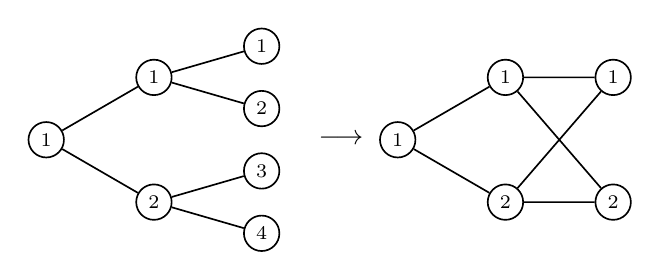
\begin{tikzpicture}[scale=0.72]
  % full tree
  \begin{scope}
    \node[nd] (r) at (0,0) {$1$};
    \node[nd] (a1) at (1.9,1.1)  {$1$};
    \node[nd] (a2) at (1.9,-1.1) {$2$};
    \node[nd] (b1) at (3.8,1.65)  {$1$};
    \node[nd] (b2) at (3.8,0.55)  {$2$};
    \node[nd] (b3) at (3.8,-0.55) {$3$};
    \node[nd] (b4) at (3.8,-1.65) {$4$};
    \draw[edg] (r) -- (a1) (r) -- (a2) (a1) -- (b1) (a1) -- (b2)
               (a2) -- (b3) (a2) -- (b4);
  \end{scope}
  \node at (5.2,0) {$\longrightarrow$};
  % recombined tree
  \begin{scope}[xshift=6.2cm]
    \node[nd] (rr) at (0,0) {$1$};
    \node[nd] (c1) at (1.9,1.1)  {$1$};
    \node[nd] (c2) at (1.9,-1.1) {$2$};
    \node[nd] (d1) at (3.8,1.1)  {$1$};
    \node[nd] (d2) at (3.8,-1.1) {$2$};
    \draw[edg] (rr) -- (c1) (rr) -- (c2) (c1) -- (d1) (c2) -- (d2)
               (c1) -- (d2) (c2) -- (d1);
  \end{scope}
\end{tikzpicture}
\end{center}

\begin{itemize}
	\item
When can we recombine nodes?
	\item
When can we assign the same value function $\QQ_{t+1}(x)$ to
each node $k$ of stage $t$?
\end{itemize}

\end{frame}

\begin{frame}
\frametitle{Nested decomposition is non-scalable}

Assume $H$ time steps, $M_t$ discrete outcomes in each stage, and relatively complete
recourse (no feasibility cut needed). The tree then has $N_t = \prod_{j=1}^t M_j$ nodes at
stage $t$.

\begin{center}
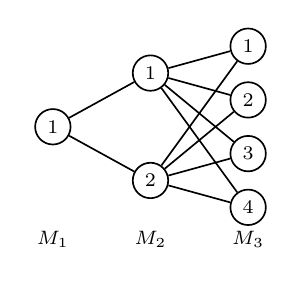
\begin{tikzpicture}[scale=0.62]
  \recombgraph{nd}{nd}
  \node[stg] at (0,-2.3) {$M_1$};
  \node[stg] at (2,-2.3) {$M_2$};
  \node[stg] at (4,-2.3) {$M_3$};
\end{tikzpicture}
\end{center}

\begin{small}
\begin{itemize}
	\item
Forward pass: $M_1 + M_1 \times M_2 + \ldots = \sum_{t = 1}^H \prod_{j = 1}^t M_j$ linear programs;
	\item
Backward pass:  $\sum_{t = 2}^{H} \prod_{j = 1}^t M_j$ linear programs.
\end{itemize}
The effort grows \textcolor{red}{exponentially} with the horizon.
\end{small}

\end{frame}

\begin{frame}
	\frametitle{Nested decomposition vs extensive form}

	The alternative to nested decomposition is the extensive form.
	\begin{itemize}
		\item
		The extensive form will not even load in memory.
		\item
		Nested decomposition will load in memory, but will not
		terminate (for large problems).
	\end{itemize}

	Nested decomposition lays the foundation for SDDP.

	\mbox{}

	As the method name suggests, we are in the context of dynamic programming.

\end{frame}

\begin{frame}
	\frametitle{Enumerating versus simulating}

\begin{center}
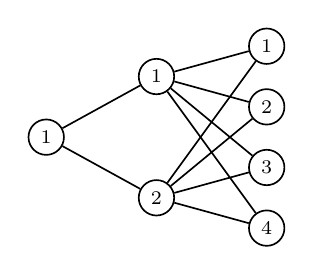
\begin{tikzpicture}[scale=0.7]
  \recombgraph{nd}{nd}
\end{tikzpicture}
\end{center}

\begin{itemize}
	\item
	Enumeration: $\{(1, 1), (1, 2), (1, 3), (1, 4), (2, 1), (2, 2), (2,
		3), (2, 4)\}$;
	\item
	Simulation (with 3 samples): $\{(1, 3), (2, 1), (1, 4)\}$.
\end{itemize}
\end{frame}

\begin{frame}
\frametitle{Making nested decomposition scalable}

Solution for the forward pass:
\begin{itemize}
	\item
in the forward pass, we simulate instead of enumerating;
	\item
this results in a probabilistic upper bound and termination
criterion.
\end{itemize}

\mbox{}

Solution for the backward pass:
\begin{itemize}
	\item
in the backward pass, we share cuts among nodes of the
same time period;
\item
this requires an assumption of \textcolor{red}{stagewise independence}.
\end{itemize}

\mbox{}

{\small \textcolor{red}{Stagewise independence}: the random vector $\xi_{t+1}$ is independent of $\xi_{[t]} = (\xi_1,\ldots, \xi_t)$ for $t = 1,\ldots, H-1$ (see for instance A. Shapiro, ``Analysis of stochastic dual dynamic programming'', European Journal of Operational Research, 209(1), 2011, pp. 63--72). Here, $\xi_1$ has a unique realization.}

\end{frame}

\begin{frame}
	\frametitle{Implications for the forward pass}

At each forward pass we solve $H-1$ subproblems along a single sampled scenario.

\begin{center}
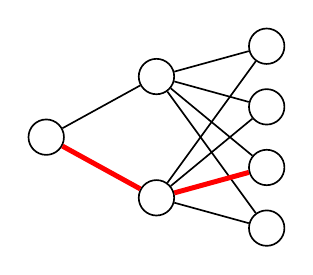
\begin{tikzpicture}[scale=0.7]
  \node[nd] (r) at (0,0) {};
  \node[nd] (a1) at (2,1.1)  {};
  \node[nd] (a2) at (2,-1.1) {};
  \node[nd] (b1) at (4,1.65)  {};
  \node[nd] (b2) at (4,0.55)  {};
  \node[nd] (b3) at (4,-0.55) {};
  \node[nd] (b4) at (4,-1.65) {};
  \draw[edg] (r) -- (a1);
  \foreach \a in {a1,a2} \foreach \b in {b1,b2,b3,b4} \draw[edg] (\a) -- (\b);
  \draw[edgsel] (r) -- (a2);
  \draw[edgsel] (a2) -- (b3);
\end{tikzpicture}
\end{center}

For $K$ Monte Carlo simulations, we solve $1 + K\times (H-1)$ linear
programs, whatever the size of the scenario tree.

\end{frame}

\begin{frame}
\frametitle{Implications for the backward pass}

Stagewise independence implies the same value function for all nodes
of stage $t$ $\Longrightarrow$ cut sharing.

\begin{center}
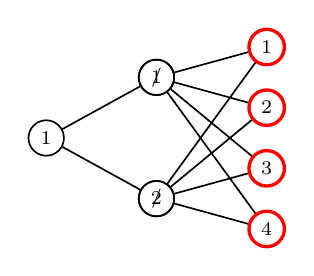
\begin{tikzpicture}[scale=0.7]
  \recombgraph{nd}{ndsel}
  \node[nd] at (2,1.1)  {$/$};
  \node[nd] at (2,-1.1) {$/$};
\end{tikzpicture}
\end{center}

For a given trial sequence $\hat{x}_{t}$, $t = 1,\ldots,H-1$, we solve
$\sum_{t=2}^{H} M_t$ linear programs, and for $K$ trial sequences,
$K\sum_{t=2}^{H} M_t$ linear programs: the effort is now
\textcolor{red}{linear} in the horizon.

\end{frame}

\begin{frame}
\frametitle{Stagewise independence is not necessary}

We can use dual multipliers in stage $t + 1$ for cuts in stage $t$
even without stagewise independence.

\mbox{}

However, each node in stage $t$ has a different value function, so
\begin{itemize}
	\item
more memory consumption;
	\item
more optimality cuts needed because we are
approximating more value functions.
\end{itemize}
With stagewise independence, we can
\begin{itemize}
	\item
get rid of the scenario tree;
	\item
work with a continuous distribution of $\xi_t$.
\end{itemize}
An intermediate solution consists in adding $\xi_{t}$ to the state vector, for instance
when the noise follows an autoregressive model.

\end{frame}

\begin{frame}
\frametitle{SDDP forward pass}

\begin{itemize}
	\item
Solve $NLSD(1, 1)$. Let $x_{1,1}$ be the optimal solution.
Initialize $\hat{x}_{1,i} = x_{1,1}$ for $i = 1,\ldots,K$.
\item
For $t = 2,\ldots, H$, $i = 1,\ldots, K$,
\begin{itemize}
	\item
sample a realization $\xi_{t,i}$ among $\xi_{t,k}$, $k = 1,\ldots,M_t$, which
determines $(c_{t,i}, h_{t,i}, T_{t-1,i})$;
\item
solve $NLSD(t, i)$ with the trial decision $\hat{x}_{t-1,i}$;
\item
store the optimal solution as $\hat{x}_{t,i}$, and the stage cost
$c_{t,i}^T\hat{x}_{t,i}$.
\end{itemize}
\end{itemize}

\mbox{}

The stage costs exclude $\theta_{t,i}$: otherwise the future would be counted twice.

\end{frame}

\begin{frame}
	\frametitle{SDDP backward pass}

\begin{itemize}
	\item
For $t = H, H - 1,\ldots, 2$, for $i = 1,\ldots, K$,
\begin{itemize}
	\item
solve $NLSD(t, k)$ with the trial decision $\hat{x}_{t-1,i}$, for $k = 1,\ldots, M_t$;
\item
compute
\begin{align*}
E_{t-1} &= \sum_{k = 1}^{M_t} p_{t,k} \pi_{t,k,i}^T T_{t-1,k}, \\
e_{t-1} &= \sum_{k = 1}^{M_t} p_{t,k} \left( \pi_{t,k,i}^T h_{t,k}
+ \sum_j \rho_{t,k,i,j} d_{t,k,j} + \sum_j \sigma_{t,k,i,j} e_{t,k,j} \right);
\end{align*}
\item
add the optimality cut
$
E_{t-1}x_{t-1} + \theta_{t-1} \geq e_{t-1}
$
to $NLSD(t - 1, k)$, $k = 1,\ldots, M_{t-1}$.
\end{itemize}
\end{itemize}
The same cut is added to every node of stage $t-1$: this is cut sharing.

\end{frame}

\begin{frame}
\frametitle{Probabilistic upper bound}

Suppose we draw a scenario $i$, that is a realization of $(\xi_{t})$, $t = 2,\ldots,H$, and
solve $NLSD(t, i)$ for $t = 1,\ldots,H$ (noting that for $t = 1$, the problem is
deterministic).
\begin{itemize}
\item
This gives $x_{t,i}$, $t = 1,\ldots,H$, with a cost $z_i = \sum_{t=1}^H c_{t,i}^Tx_{t,i}$.
\item
Each $(x_{t,i},\ t = 1,\ldots,H)$ is feasible but not necessarily optimal, so the expected
cost $\mu = \EE[z_i]$ of the current policy is an upper bound on the optimal value.
\item
Consider $K$ independent scenarios, and the mean cost
$
\overline{z}_K = \frac{1}{K} \sum_{i=1}^K z_i.
$
By the Central Limit Theorem,
$$
\sqrt{K}\,(\overline{z}_K - \mu) \overset{\mathcal{D}}{\rightarrow} N(0, \sigma^2),
\quad \text{i.e., } \overline{z}_K \approx N\left(\mu, \frac{\sigma^2}{K}\right).
$$
\item
$\overline{z}_K$ only estimates that upper bound: a realization of $\overline{z}_K$ may well
fall below the optimal value.
\end{itemize}

\end{frame}

\begin{frame}
\frametitle{Bounds and termination criterion}

{\small
After solving $NLSD(1, 1)$ in a forward pass we can compute a lower bound $z_{LB}$
as the objective function value of $NLSD(1, 1)$: the cuts are an outer approximation of the
expected cost-to-go, hence $NLSD(1,1)$ is a relaxation of the original problem.

\mbox{}

Terminate if $z_{LB} \in (\overline{z}_K - \Phi^{-1}(1-\alpha/2) \hat{s}/\sqrt{K}, \overline{z}_K + \Phi^{-1}(1-\alpha/2) \hat{s}/\sqrt{K})$, where $\Phi(\cdot)$ is the cumulative distribution of a Normal(0,1), and $\alpha$ is a confidence level set by the user. Typically, $\alpha = 0.05$. Since $z_{LB}$ is a lower bound, only the left inequality really matters.

\mbox{}

How to ensure a $1\%$ optimality gap with $95\%$ confidence?
Choose $K$ such that $\Phi^{-1}(1-\alpha/2)\hat{s}/\sqrt{K} \approx 0.01 \overline{z}_K$. Using the empirical standard deviation
$
\hat{s} = \sqrt{\frac{1}{K-1} \sum_{i=1}^K (z_i - \overline{z}_K)^2},
$
this leads to
$$
K = \left( \frac{\Phi^{-1}(1-\alpha/2)\hat{s}}{0.01\, \overline{z}_K}\right)^2.
$$
The criterion is optimistic: with a small $K$ the confidence interval is wide, and the
lower bound enters it long before the policy is optimal.
}

\end{frame}

\begin{frame}
\frametitle{SDDP algorithm}

\begin{small}
\begin{algorithmic}[1]
\State Set $K$, $\alpha$, the maximum number of iterations, and start with no cut.
\Repeat
  \State \textbf{Forward pass}: solve $NLSD(1,1)$, set $z_{LB}$ to its optimal value;
  \State \quad simulate $K$ scenarios, collect the trial solutions $\hat{x}_{t,i}$ and the costs $z_i$;
  \State \quad compute $\overline{z}_K$ and $\hat{s}$.
  \If{$z_{LB} \geq \overline{z}_K - \Phi^{-1}(1-\alpha/2)\hat{s}/\sqrt{K}$}
    \State \textbf{stop}: the gap is not statistically significant.
  \EndIf
  \State \textbf{Backward pass}: for $t = H,\ldots,2$ and $i = 1,\ldots,K$, solve the $M_t$
  \State \quad subproblems at $\hat{x}_{t-1,i}$ and add the resulting cut to stage $t-1$.
\Until{the iteration limit is reached}
\end{algorithmic}
\end{small}

{\small The lower bound is deterministic and non-decreasing; the upper bound is statistical.}

\end{frame}

\begin{frame}
\frametitle{Numerical illustration}

{\small Hydro-thermal scheduling, $H = 6$ stages, $M_t = 4$ inflow outcomes
($1024$ scenarios), $K = 5$ forward passes per iteration.}

\begin{center}

\includegraphics[height=0.48\textheight]{sddp_convergence.pdf}
\end{center}

{\small The lower bound reaches the optimal value of the extensive form after a few
iterations, while the simulated cost keeps oscillating around it.}

\end{frame}

\begin{frame}
\frametitle{Numerical illustration: the cuts}

\begin{center}

\includegraphics[height=0.50\textheight]{sddp_value_function.pdf}
\end{center}

{\small Each cut lies below the exact expected cost-to-go, and the approximation is tight
only where the forward passes went: the value function is never learned everywhere.
Computed with \texttt{code/SDDP\_from\_scratch.ipynb}.}

\end{frame}

\begin{frame}
\frametitle{References}

\begin{itemize}
\item
M.V.F. Pereira and L.M.V.G. Pinto, ``Multi-stage stochastic optimization applied to energy
planning'', \emph{Mathematical Programming} 52, 359--375, 1991.
\item
A. Shapiro, ``Analysis of stochastic dual dynamic programming method'', \emph{European
Journal of Operational Research} 209(1), 63--72, 2011.
\item
J.R. Birge and F. Louveaux, \emph{Introduction to Stochastic Programming}, 2nd edition,
Springer, 2011 (Chapter 7).
\item
O. Dowson and L. Kapelevich, ``SDDP.jl: a Julia package for stochastic dual dynamic
programming'', \emph{INFORMS Journal on Computing} 33(1), 27--33, 2021.
\item
A. Papavasiliou, lecture notes on SDDP,
\url{https://ap-rg.eu/wp-content/uploads/2020/05/SDDP.pdf}.
\end{itemize}

\end{frame}

\end{document}
